\documentclass{article}
\usepackage{subfig}
\usepackage[dutch]{babel}
\usepackage{minutes}
\usepackage{graphicx}
\usepackage{float}

\title{Notulen 011 overleg team 33}
\author{Stefan}
\minutesstyle{header=table, vote=list, contents=true, columns={1}}

\begin{document}
%\selectlanguage{dutch}

\begin{Minutes}{Overleg 011 team 33}
\participant{Guus Bonnema, Stefan Versluys}
\minutesdate{1 november 2014}
\location{Skype}

\maketitle% This is where LaTeX makes the title

\topic{Bespreken aanpak domeinanalyses}

Uitleg Stefan: 
\begin{itemize}
\item 90pct van het DA document zal over de structuur gaan van combinatorial objects de rest over de manier van oa. grafisch voorstelling.
\item Informatie tot nu toe is bekomen op basis de documentatie, feedback van Freek en van het analyseren van in- en output van het WickedXmas tool.
\item Afbakening van het DA gebied waarin de data structuren voorkomen reikt van wck, fjson tot de C library file (zie figuur 1, groene kader).
\item Op basis van deze analyse gezien dat primitieven deel moeten uitmaken van deze DA.
\item WickedXmas is niet meer dan een grafische en statische editor , input is wck(fjson) , output is C library file.
\end{itemize}

\begin{figure}[t]
  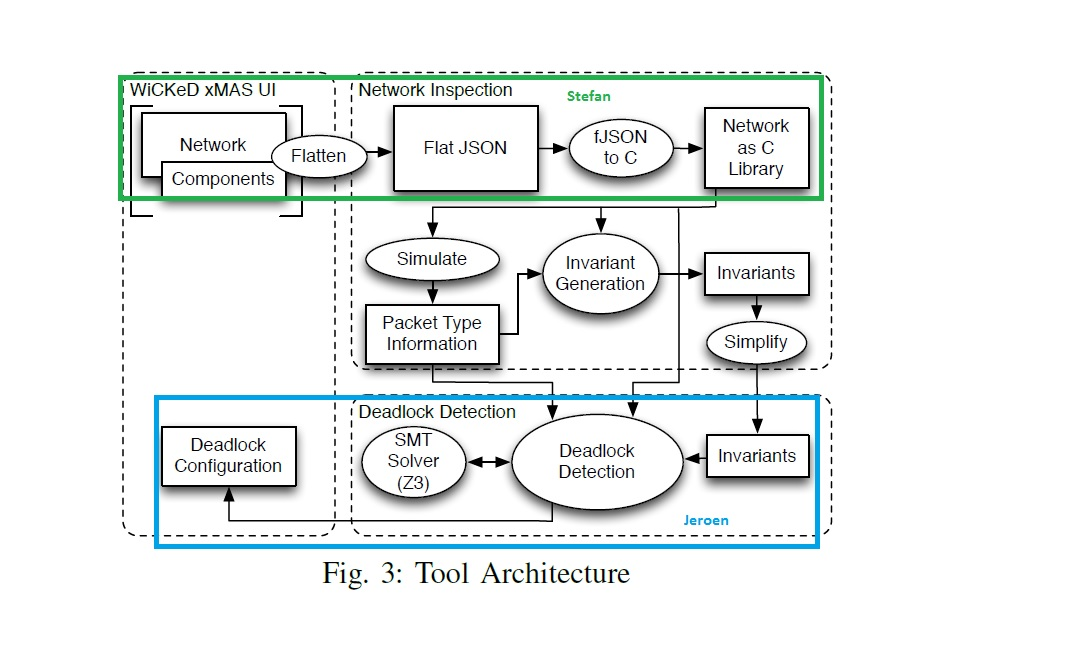
\includegraphics[width=\textwidth]{da_zones}
  \caption{Vermoedelijke afbakening DA Jeroen en Stefan}
\end{figure}



Bemerkingen:
\begin{itemize}
\item Focus op de achterliggende structuur, het grafisch deel is makkelijker nadien aan te passen  $\rightarrow$ ok, dit was de bedoeling, betreft enkel de grafische voorstelling van een combinatorial object, meer bepaalt of de huidige voldoet of niet.
\item Analyse ook vanuit het perspectief of we al deze tussenstructuren wel nodig hebben , kan de nieuwe WickedXmas editor eventueel rechtstreeks op een target structuur werken. $\rightarrow$ ok , redundante informatie kan leiden tot inconsistentie, goed idee.
\end{itemize}

\newpage
Uitleg Guus: 
\begin{itemize}
\item Blijkt een enorm aanbod te zijn van mogelijke GUI tools, Qt is lang niet de enige geschikte kandidaat, dit levert meer werk dan gedacht.
\item Software \underline{moet} free zijn en blijven (bijkomende requirement).
\item GUI selecteren op basis van free (open source), moet voldoen aan onze requirements, actieve community met voldoende ontwikkelaars.
\item Het DA document zal beschreven worden op basis van de conclusie, de keuze wordt beargumenteerd op basis van de in de analyse onderzochte opties.
\item Bedoeling is om tot een selectie te komen van drie GUI toolkits en die met elkaar te vergelijken.
\end{itemize}

Bemerkingen:
\begin{itemize}
\item Kijk je dan ook naar eventuele ondersteuning van versiebeheer bijvoorbeeld met git? $\rightarrow$ Dit is in principe iets wat steeds aanwezig is en is enkel van belang voor onze source code , niet van de GUI tool op zich.
\item Moet er nadien eventueel tijd gepland worden om de tool te leren gebruiken? $\rightarrow$ Vele tools tegenwoordig zijn zo omvangrijk dat je ze niet zomaar op voorhand kunt bestuderen, vaak komt het er op neer dat het voldoende is ervaring te hebben met dergelijke tools , aan de slag gaat en voor zaken die niet duidelijk zijn hulp vraagt of enkel dat deel bestudeert en uitprobeert. 
\end{itemize}


\topic{Vragen en afspraken}

\begin{itemize}
\item Stefan stuurt gemeenschappelijke vraag naar Freek in verband met de stappen om van fjson tot c te komen, waarom de keuze voor al deze tussenstappen? (Het vermoeden bestaat dat WickedXmas C code levert omdat het resultaat ook op snelle hardware moet kunnen geverifieerd worden) (*)
\item DA's regelmatig pushen.
\item Stefan en Guus kunnen op 8 november niet naar Eindhoven , kan Jeroen eventueel?
\item Volgende skype sessie is woensdag 5 november om 19h.
\item Minutes worden vanaf nu op de master gepusht, de branch plan bestaat niet meer.
\end{itemize}
(* pag1 links onder 13toolxmas.pdf) betreft xmas netwerk: "From this high-level model, invariants can be derived and input to a hardware model-checker, e.g. ABC [3], to speed-up verification."

\end{Minutes}
\end{document}
